%% Copernicus Publications Manuscript Preparation Template for LaTeX Submissions
%% ---------------------------------
%% This template should be used for copernicus.cls
%% The class file and some style files are bundled in the Copernicus Latex Package, which can be downloaded from the different journal webpages.
%% For further assistance please contact Copernicus Publications at: production@copernicus.org
%% https://publications.copernicus.org/for_authors/manuscript_preparation.html

%% copernicus_rticles_template (flag for rticles template detection - do not remove!)

%% Please use the following documentclass and journal abbreviations for discussion papers and final revised papers.

%% 2-column papers and discussion papers
\documentclass[gc, manuscript]{copernicus}



%% Journal abbreviations (please use the same for discussion papers and final revised papers)


% Advances in Geosciences (adgeo)
% Advances in Radio Science (ars)
% Advances in Science and Research (asr)
% Advances in Statistical Climatology, Meteorology and Oceanography (ascmo)
% Annales Geophysicae (angeo)
% Archives Animal Breeding (aab)
% ASTRA Proceedings (ap)
% Atmospheric Chemistry and Physics (acp)
% Atmospheric Measurement Techniques (amt)
% Biogeosciences (bg)
% Climate of the Past (cp)
% DEUQUA Special Publications (deuquasp)
% Drinking Water Engineering and Science (dwes)
% Earth Surface Dynamics (esurf)
% Earth System Dynamics (esd)
% Earth System Science Data (essd)
% E&G Quaternary Science Journal (egqsj)
% Fossil Record (fr)
% Geochronology (gchron)
% Geographica Helvetica (gh)
% Geoscience Communication (gc)
% Geoscientific Instrumentation, Methods and Data Systems (gi)
% Geoscientific Model Development (gmd)
% History of Geo- and Space Sciences (hgss)
% Hydrology and Earth System Sciences (hess)
% Journal of Micropalaeontology (jm)
% Journal of Sensors and Sensor Systems (jsss)
% Mechanical Sciences (ms)
% Natural Hazards and Earth System Sciences (nhess)
% Nonlinear Processes in Geophysics (npg)
% Ocean Science (os)
% Primate Biology (pb)
% Proceedings of the International Association of Hydrological Sciences (piahs)
% Scientific Drilling (sd)
% SOIL (soil)
% Solid Earth (se)
% The Cryosphere (tc)
% Web Ecology (we)
% Wind Energy Science (wes)


%% \usepackage commands included in the copernicus.cls:
%\usepackage[german, english]{babel}
%\usepackage{tabularx}
%\usepackage{cancel}
%\usepackage{multirow}
%\usepackage{supertabular}
%\usepackage{algorithmic}
%\usepackage{algorithm}
%\usepackage{amsthm}
%\usepackage{float}
%\usepackage{subfig}
%\usepackage{rotating}


% The "Technical instructions for LaTex" by Copernicus require _not_ to insert any additional packages.
%
\usepackage{algorithmic}
\usepackage{algorithm}


\begin{document}

\title{Historical Soil Organic Carbon Budget}


\Author[1]{Kristine}{Karstens}
\Author[1]{Benjamin Leon}{Bodirsky}
\Author[1]{Alexander}{Popp}


\affil[1]{Potsdam-Institut of Climate Impacts Research, Potsdam,
Germany}

%% The [] brackets identify the author with the corresponding affiliation. 1, 2, 3, etc. should be inserted.



\runningtitle{R Markdown Template for Copernicus}

\runningauthor{Nüst et al.}


\correspondence{Kristine\ Karstens\ (kristine.karstenst@pik-potsdam.de)}



\received{}
\pubdiscuss{} %% only important for two-stage journals
\revised{}
\accepted{}
\published{}

%% These dates will be inserted by Copernicus Publications during the typesetting process.


\firstpage{1}

\maketitle


\begin{abstract}
SOC one of larges c sinks on earth (3 times larger biospehre pool).
Agricultural management leads to a depletion of soil organic crabon.
However this depletion of soil organic carbon (SOC) pools are so far not
well represented in global assessments of historic carbon emissions.
While SOC models often represent well the biochemical processes that
lead to the accumulation and decay of SOC, the management decisions
driving these biophysical processes are still little investigated. Here
we create a spatial explicit data set for crop residue and manure
management on cropland based on global historic production (FAOSTAT) and
land-use (LUH2) data and combine it with the IPCC Tier 2 approach to
create a half-degree resolution soil organic carbon budget on mineral
soils. We estimate that due to arable farming soils have lost over (?)
GtOC of which (??) GtOC have been released within the period 1990-2010.
Tier 2 IPCC methodolgy estimates higher soil organic carbon losses than
Tier 1 methods, which may origin from \ldots{} . We also find that SOC
is very sensity to management decision such as residue recycling
indicating the nessessity to incorporated better management data in soil
models.
\end{abstract}


\copyrightstatement{The author's copyright for this publication is
transferred to institution/company.}


\newpage

\introduction

Introduction text goes here. You can change the name of the section if
neccessary using
\texttt{\textbackslash{}introduction{[}modified\ heading{]}}. \newpage

\section{Method (50)}

\hypertarget{sec:carbonbudget}{%
\subsection{Carbon Stocks following (new) Tier 2 method
(50)}\label{sec:carbonbudget}}

Following the tier 2 approach of the refinement of IPCC guidelines
vol.~4 (\citet{ipcc_2019_2019}), we calculate annual land use type
specific soil organic carbon stocks for cropland, pastures and natural
vegetation on half-degree resolution for the period of 1965 to 2010
based on the following three steps: (1) Calculating the land use
(sub-)type specific steady-states and decay rates for SOC stocks given
the current biophysical, climatic and agronomic conditions, (2)
accounting for land conversation effects by transferring SOC between
land use types and (3) updating SOC stocks based on the previous stock,
the steady-state and the decay rate.

\subsubsection{Steady-state SOC stocks and decay rates}

In a simple first order kinetic approach the steady-state soil organic
carbon stocks \(SOC^{eq}\) are given by \begin{equation}
SOC^{eq} =\frac{C^{\textrm{in}}}{k}
\label{eq:inoutflow}
\end{equation} with \(C^{\textrm{in}}\) being carbon inputs to the soil
and \(k\) denoting the soil organic carbon decay rate. We use for our
calculations the steady-state method of the refinement of the IPCC
guidelines vol.~4 (\citet{ipcc_2019_2019}) for mineral soils, which
assume three soil carbon sub-pools (active, slow and passive) and
entangled dynamics between them. Carbon inflow to each sub-pool (see
@ref(sec:carboninputs)) and decay rates (see @ref(sec:tier2)) of each
sub-pool are still the key components to determining steady-state SOC
stocks.

\hypertarget{sec:carboninputs}{%
\subsubsection{Carbon Inputs to the Soil}\label{sec:carboninputs}}

We account for different carbon input sources depending on the land use
type (see table @ref(tab:datasourceinputs)). Following the IPCC
methodology carbon inputs are disaggregated into metabolic and
structural components depending on their lignin and nitrogen content
(see @ref(ipcc\_2019\_2019)). For each component the sum over all carbon
input sources is allocated to the respective SOC sub-pools via transfer
coefficients. This implies that not only the amount of carbon, but also
their structural composition is determining the effective inflow. Data
sources for all considered carbon inputs as well as for lignin and
nitrogen content can be found in table @ref(tab:datasourceinputs).

 \begin{table*}[h]
 \caption{Type and data sources for carbon inputs to different land use types}
 \begin{tabular}{l l l l}
 \tophline
  Land use types   & source of carbon inputs & data source & nitrogen and lignin content \\
 \middlehline
 \multirow{3}{*}{Cropland} & residues & FAOSTAT, LPJmL4 [2, sec:residues] & default values given by [2]  \\
                            & dead below ground biomass of crops & FAOSTAT, LPJmL4 [2, sec:residues] & default values given by [2] \\
                            & manure & FAOSTAT, Isabelle [2, sec:manure] & default values given by [2] \\
                            \hline
 \multirow{2}{*}{Pasture}  & annual litterfall & LPJmL4 [3] & default values given by [2] \\ 
                            & manure  & FAOSTAT, Isabelle [2, sec:manure] & default values given by [2] \\
                            \hline
  Natural vegetation        & annual litterfall & LPJmL4 [4]& \begin{minipage}[t]{0.28\columnwidth}\raggedright\strut Nitrogen and lignin content of tree compartments used in CENTURY [4] \strut \end{minipage}\tabularnewline
 \bottomhline
 \end{tabular}
 \label{tab:datasourceinputs}
 \belowtable{}
 \end{table*}

\hypertarget{sec:tier2}{%
\subsubsection{Soil Organic Carbon decay (300)}\label{sec:tier2}}

The sub-pool specific decay rates are influenced by climatic conditions,
biophysical and biochemical soil properties as well as management
factors that vary over time (t) and space (i). Following the
steady-state method of the refinement of the IPCC guidelines vol.~4
(\citet{ipcc_2019_2019}) for mineral soils we consider temperature
(temp), water (wat), sand fraction (sf) and tillage (till) effects to
account for spatial variation of decay rates. Thus \(k_{sub}\) is given
by

\begin{equation}
\begin{aligned}
& k_{active,t,i}  & = &~ k_{active}  ~ &\cdot~ temp_{t,i} ~ &\cdot~ wat_{t,i} ~ &\cdot~ till_{t,i} ~ & \cdot~ sf_{t,i}\\
& k_{slow,t,i}    & = &~ k_{slow}    ~ &\cdot~ temp_{t,i} ~ &\cdot~ wat_{t,i} ~ &\cdot~ till_{t,i} ~ &\\
& k_{passive,t,i} & = &~ k_{passive} ~ &\cdot~ temp_{t,i} ~ &\cdot~ wat_{t,i} ~ & ~ &
\label{eq:decayrates}
\end{aligned}
\end{equation}

For cropland we distinguish the effect of different tillage (see
@ref(\#sec:tillage)) and irrigation (see @ref(\#sec:irrigation))
practices on decay rates, whereas on pastures and natural vegetation, we
assume rainfed and non-tilled conditions. Data sources as well as
considered effects for each land use types are shown in table
@ref(tab:datasourcedecay). To account for variations of decay rates
within each grid cell due to different tillage and irrigation regimes,
average rates based on area shares are calculated.

 \begin{table*}[h]
 \caption{Type and data sources for carbon inputs to different land use types}
 \begin{tabular}{l l l l}
 \tophline
  Land use types   & type of decay driver & parameter use to represent driver & data source \\
 \middlehline
 \multirow{2}{*}{all} & Soil quality & Sand fraction of the first 0-30 cm &  [SoilGrids]  \\
                      \cline{2-4}
                      
                      & Mircobial activity & air temperature & [CRUp4.0] \\
                      \cline{2-4}
                      
                      & Water restriction & precipitation \& potential evapotranspiration & [CRUp4.0] \\
                      \cline{1-4}
\multirow{2}{*}{\begin{minipage}[t]{0.2\columnwidth}\raggedright\strut Cropland\\(additionally)\strut\end{minipage}} & Water restriction*  & irrigation  & [sec:irrigation] \\ 
                      \cline{2-4}
                      
                      & Soil disturbance & tillage & [sec:tillage] \\
 \bottomhline
 \end{tabular}
 \label{tab:datasourcedecay}
 \belowtable{}
 \end{table*}

\subsubsection{SOC transfer between land use types}

We calculate SOC stocks based on the area shares of land use types (lut)
within the half-degree grid cells (i). If land is converted from one
land use type into others (!lut), the respective share of the SOC stocks
is reallocated. We account for land conversion at the beginning of each
time step \(t\) by calculating a preliminary stock \(SOC_{lut,t*}\) via

\begin{equation}
SOC_{lut,t*} = SOC_{lut,t-1} - \frac{SOC_{lut,t-1}}{A_{lut,t-1}} \cdot  AR_{lut,t} + \frac{SOC_{!lut,t-1}}{A_{!lut,t-1}} \cdot  AE_{lut,t} \qquad \forall sub, i  
\label{eq:ctransfer}
\end{equation}

with \(A\) being the area, \(AR\) the area reduction and \(AE\) the area
expansion for a given land use type \(lut\). Note that \(!lut\) denotes
the sum over all other land use types, which decreases in the specific
time step \(t\). Data sources and methodology on land use states and
changes are described in @ref(sec:landuse).

\subsubsection{Total SOC stocks}

Carbon stocks \(SOC\) for each sub-pool (sub) converge towards the
calculated steady-state stock \(SOC^{eq}\) for each land-use types
(lut), each sub-pool (sub) and each annual time step (t) as represented
in equation @ref(eq:steadystate).

\begin{equation}
SOC_{t} = SOC_{t-1} + (SOC^{eq}_{t} - SOC_{t-1}) \cdot k_{t} \cdot 1\unit{a} \qquad \forall lut, sub, i.
\label{eq:steadystate}
\end{equation}

The global SOC stock for each time step can than be calculated via

\begin{equation}
SOC_{t} = \sum_{i} \underbrace{\sum_{lut} \overbrace{\sum_{sub} SOC_{lut, sub, t, i}.}^{\text{$SOC_{lut, t, i}$ - land use type specific SOC stock within cell}}}_{\text{$SOC_{t, i}$ - total SOC stock within cell}}
\label{eq:totalstock}
\end{equation}

\subsubsection{Initialisation of SOC pools}

To initialize all SOC sub-pools we assume that

\newpage

\hypertarget{sec:tier1}{%
\subsection{Carbon Budget following Tier 1 (150)}\label{sec:tier1}}

Additionally to the tier 2 approach of the refinement of IPCC guidelines
vol.~4 (\citet{ipcc_2019_2019}), we also estimate SOC pools using the
IPCC tier 1 approach of IPCC guidelines vol.~4 (\citet{ipcc_2006_2006})
for comparison. Here, stocks are estimated via stock change factors
given by the IPCC for the topsoil (0-30 cm) and based on a review of
measurement data. The factors differentiate different crop and
management systems reflecting different dynamics under changed in- and
outflows without explicitly tracking these. The SOC stocks as thus
calulated

\begin{equation}
SOC_{\text{target}} = \sum_{c,s,i} SOC_{\text{ref}_{c,s,i}} \cdot F_{\text{LU}_{c,s,i}} \cdot F_{\text{MG}_{c,s,i}} \cdot F_{\text{I}_{c,s,i}} \cdot A_{c,s,i}
\label{eq:tier1}
\end{equation}

\textless!- also include an equation here --\textgreater{} \textless!-
even if there are just ``copied'' out of te guidelines so to say?
--\textgreater{} \textless!- more details will follow - how deep to go?
--\textgreater{}

\hypertarget{sec:agrimanagement}{%
\subsection{Agricultural management data on 0.5 degrees
(50)}\label{sec:agrimanagement}}

\hypertarget{sec:landuse}{%
\subsubsection{Landuse and Landuse Change (150)}\label{sec:landuse}}

Land use patterns are based on the Land-Use Harmonization 2 (LUH2,
\citep{LUH2}) data set, which we aggregate from quarter degree to half
degree resolution. We disaggregate the five different cropland
subcategories (c3ann, c3per, c4ann, c4per, c3nfx) of LUH2 into our 17
crop groups, assuming relative shares for each gridcell based on the
country and year specific area shares of FAOSTAT data (\citep{FAOSTAT})
(see @ref(append:Table\_luh2fao2mag) for more details on the crop type
mapping). Land use transitions are calculated as net area differences of
the land use data on half-degree.

\subsubsection{Crop, Crop Residues and Pasture Production (300)}

Using half-degree yield data from LPJmL (\citep{LPJmL4_1}) as well as
half-degree cropland patterns (see @ref(\#sec:landuse)) we compile crop
group specific half-degree production patterns. We calibrate cellular
yields with one country-level calibration factor for each crop group to
meet historical FAOSTAT production (\citep{FAOSTAT}). Note that by using
physical cropland areas we account for multiple crop harvest events as
well as for fallows.

Crop residue production and management is based on a revised methodology
of (\citep{bodirsky2012}) and will be explained in key aspects again due
to its central role for soil carbon modelling. Starting from crop
production estimates of the harvested organs and their respective crop
area, we estimate above-ground (ag) and below-ground (bg) residual
biomass using yield-dependent harvest indices and shoot:root ratios. We
assume that all bg residues are recycled to the soil, whereas ag
residues can be burned or harvested for other purposes such as feeding
animals (\citep{weindl}), fuel or for material use.

A fixed share of the ag residues is assumed to be burned on field, which
depends on the per-capita income of the country. Following
\citep{smil1999}) we assume 25\% burn share for low-income countries
according to worldbank definitions (\(<\,1000\,\tfrac{USD}{yr}\)), 15\%
for high-income (\(>\,10000\,\tfrac{USD}{yr}\) and linearly interpolate
shares for all middle-income countries depending on their per-capita
income.

Residue demand for feed is based on country and livestock specific feed
basekts (see \citep{weindl}) taking available ag residual biomass as
well as livestock productivity into account. The three residue groups
(straw, high-lignin and low-lignin residues) of the feed baskets are
disaggregated to the crop groups, using\ldots. (see
@ref(append:Table\_kcr2kres)). \textless-- its a disggregation, no
--\textgreater{}

We estimated a material use share for the straw residues group of 5\%
and a fuel demand share demand of 10\% \textless-- only for straw, or
for all groups? --\textgreater{} in low income countries.

The remaining ag residues as well as all bg residues are assumend to be
recycled to the soil.

Using livestock production statistics as well as feed mix assumptions as
describted in (\citep{weindl}) we estimating country specific pasture
production. Following the same approach as for crop production we
disaggregate and calibrate half-degree pasture production pattern from
grass yields from LPJmL and pasture area and rangeland patterns ( (see
@ref(\#sec:landuse))) to derive half-degree pasture production patterns.

To transform dry matter estimates into carbon, we compiled crop group
and plant part specific carbon to dry matter (c:dm) ratios (see
@ref(append:Table\_c2dm)) (\citet{Ma2018}).

\subsubsection{Livestock Distribution and Manure Excretion (300)}

To disaggregate country level FAOSTAT livestock production values to
half-degree pattern, we use the following rule based assumptions which
were inspired by the approach of \citep{gilbert}.

For poultry, egg and monogastric meat production we divide into
intensive and extensive production systems based on a per-capita income
of the country. For low-income countries according to worldbank
definitions (\textless1000 USD/yr), we assume extensive production
systems. We located them according to (built-up areas shares\textbar{}
population shares) based on the idea that these animals are held in
households, subsistence or small-holder farming systems.

\begin{itemize}
\item
  Intensive production is distributed within a country using the crop
  production (excluding 2nd generation bioenergy crops) share, assuming
  that feed availability is the most driving factor for livestock
  location.
\item
  For dairy and ruminated meat production we
\item
  splot into pasture fed and non-pasture fed fractions based on the
  aggregated feed mix within a country (explain rules)
\end{itemize}

\begin{itemize}
\item
  Pasture fed animals are distributed to half-degree cells according to
  the pasture production shares of that cell within a country (not
  methodologically clear description).
\item
  Non-pasture fed animals are distributed again using crop production
  (excluding 2nd generation bioenergy crops) shares (not clear, either).
\end{itemize}

We calculate excretions by first estimating the nitrogen balance of the
livestock system (\citep{bodirsky1012}) on the basis of comprehensive
livestock feed baskets ({[}weindl{]}), assuming that all nitrogen in
protein feed intake, minus the nitrogen in the slaugher mass, is
excreted. Carbon in excreted manure is estimated by applying fixed C:N
ratios (given by \citep[(][]{ipcc_2019_2019}). What about animal waste
management losses?

\subsubsection{Irrigation (100)}

Simple growing period calculations together with irrigation shares of
LUH2v2 are used (BB: you dont like d's, on't you) to estimate water
effects on decay rates.

\subsubsection{Tillage (100)}

Tillage data sets of {[}Vera, others{]} together with rules are used to
drive tillage effect on decay rates. \newpage

\section{Results}

\begin{figure}
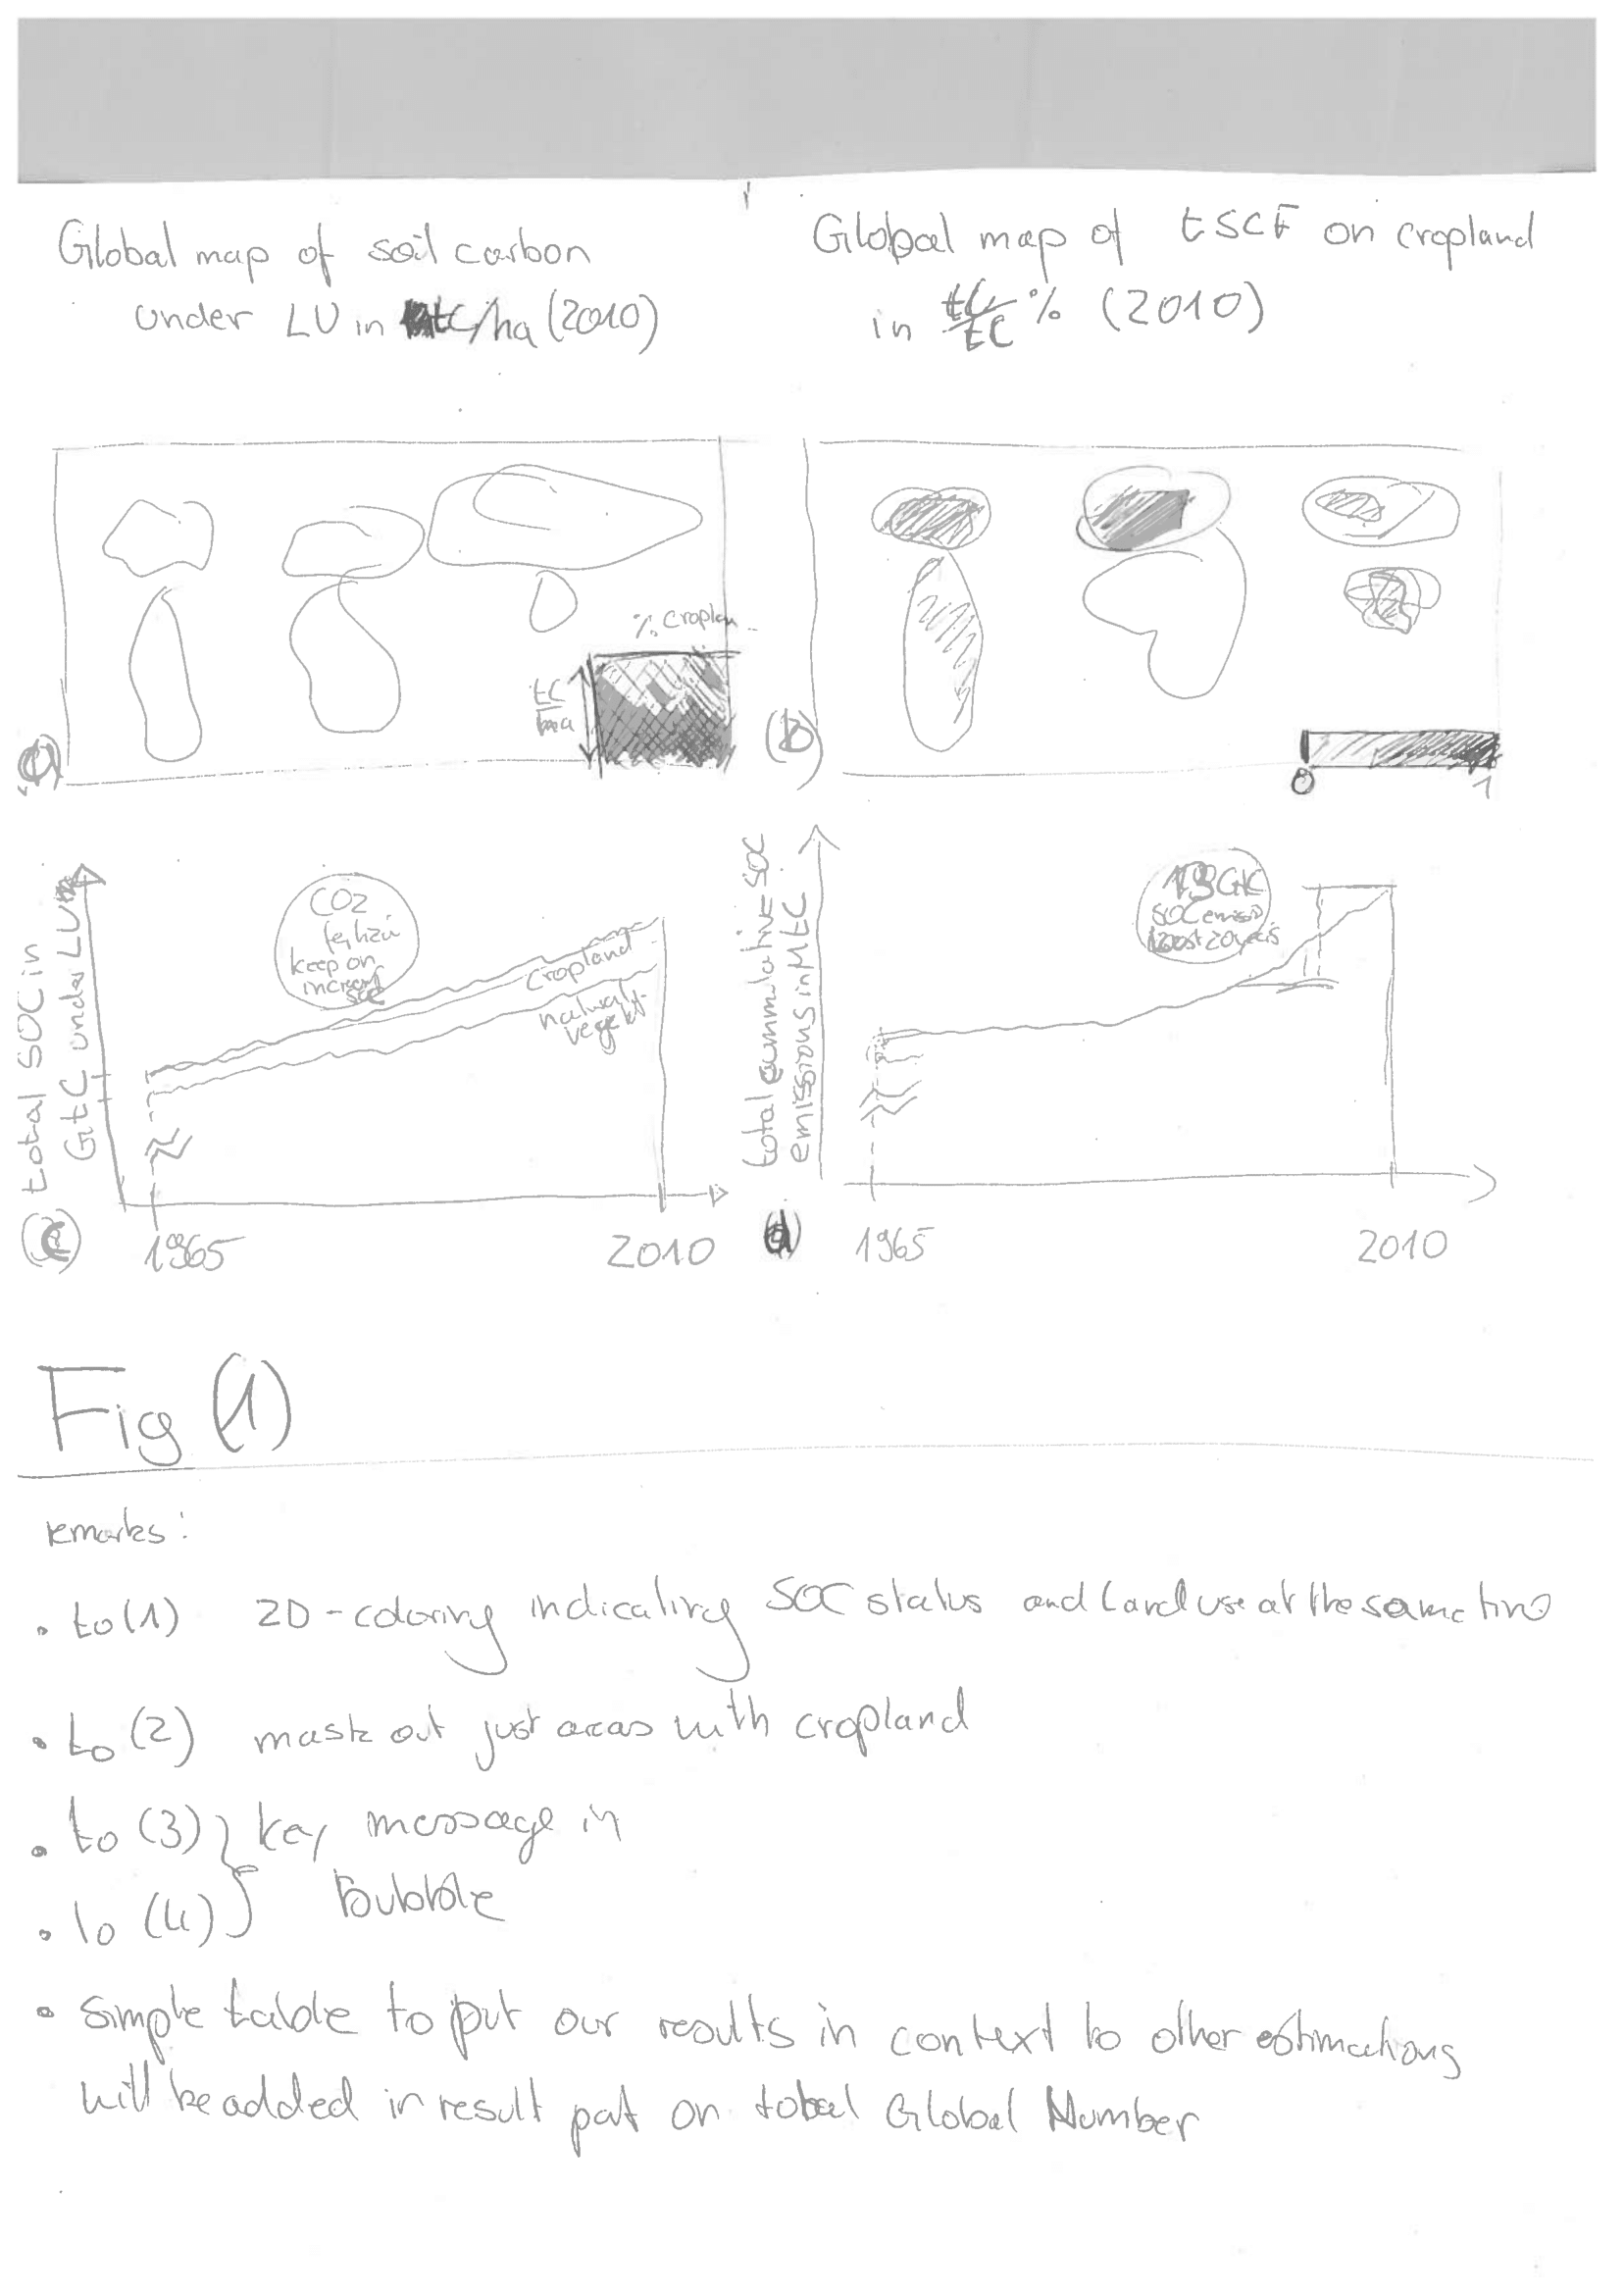
\includegraphics[width=12cm]{images/figs_draft-1} \caption{two column figure}\label{fig:unnamed-chunk-6}
\end{figure}

\begin{figure}
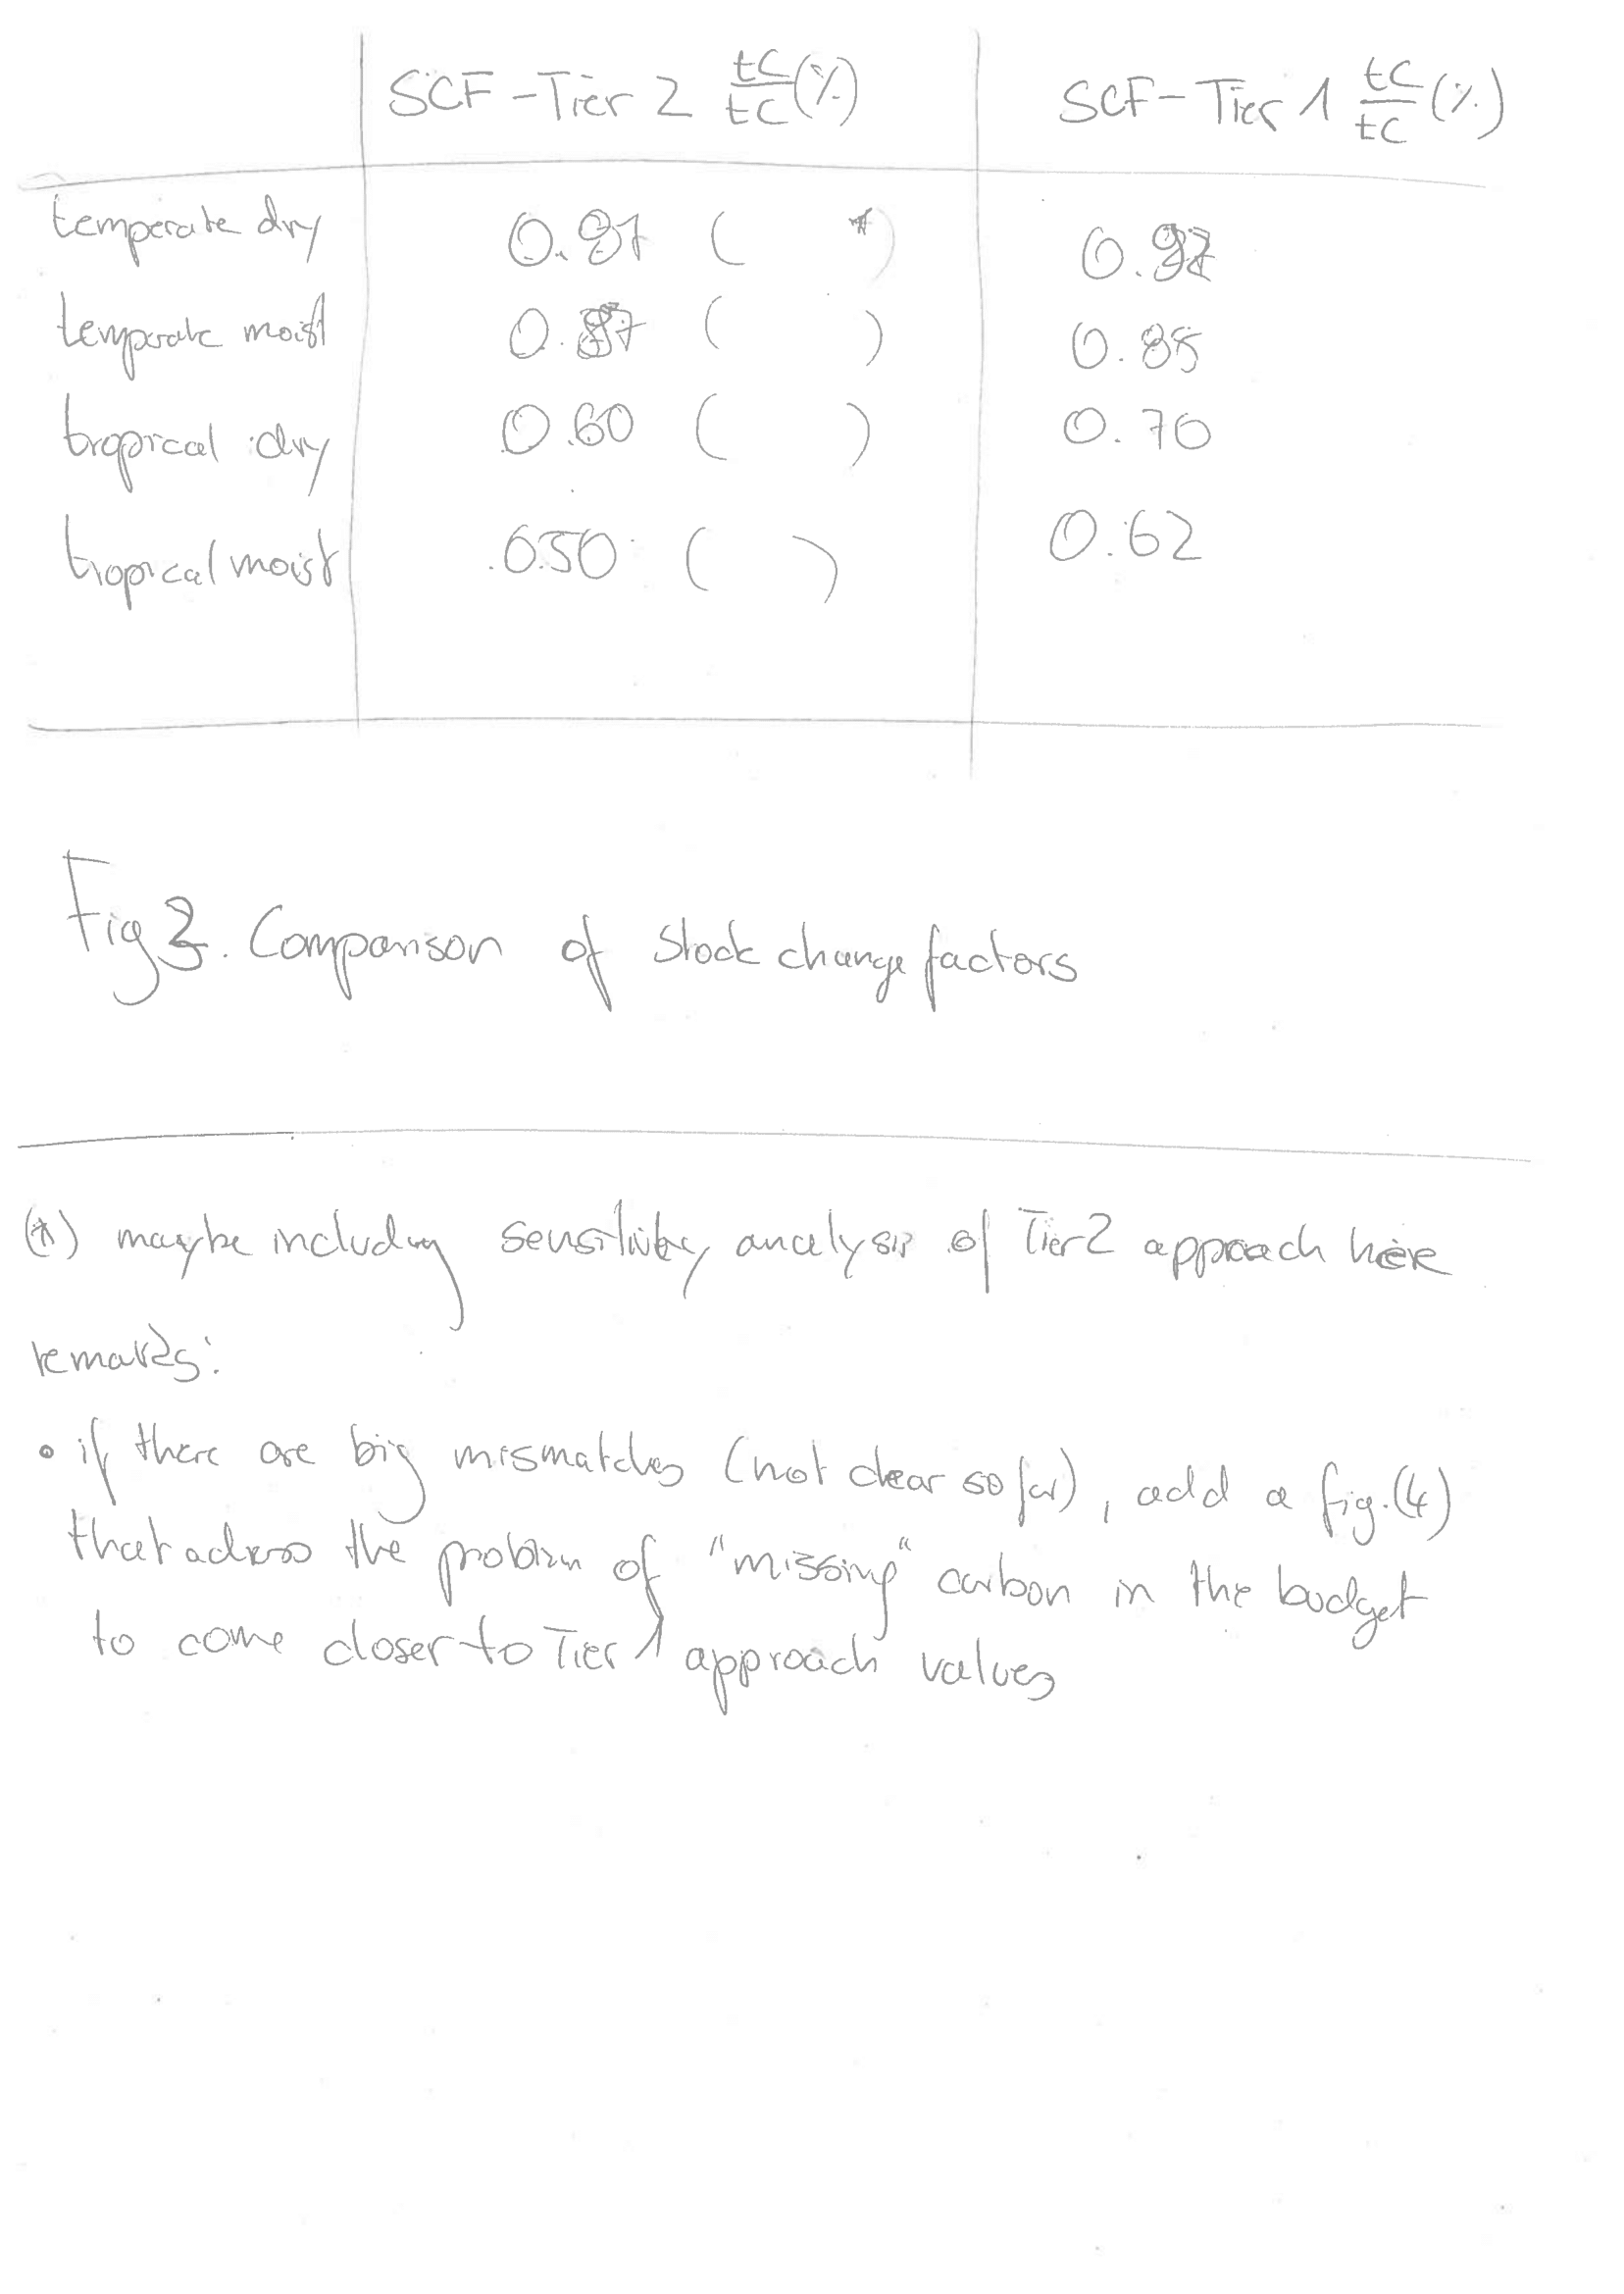
\includegraphics[width=12cm]{images/figs_draft-2} \caption{two column figure}\label{fig:unnamed-chunk-7}
\end{figure}

\begin{figure}
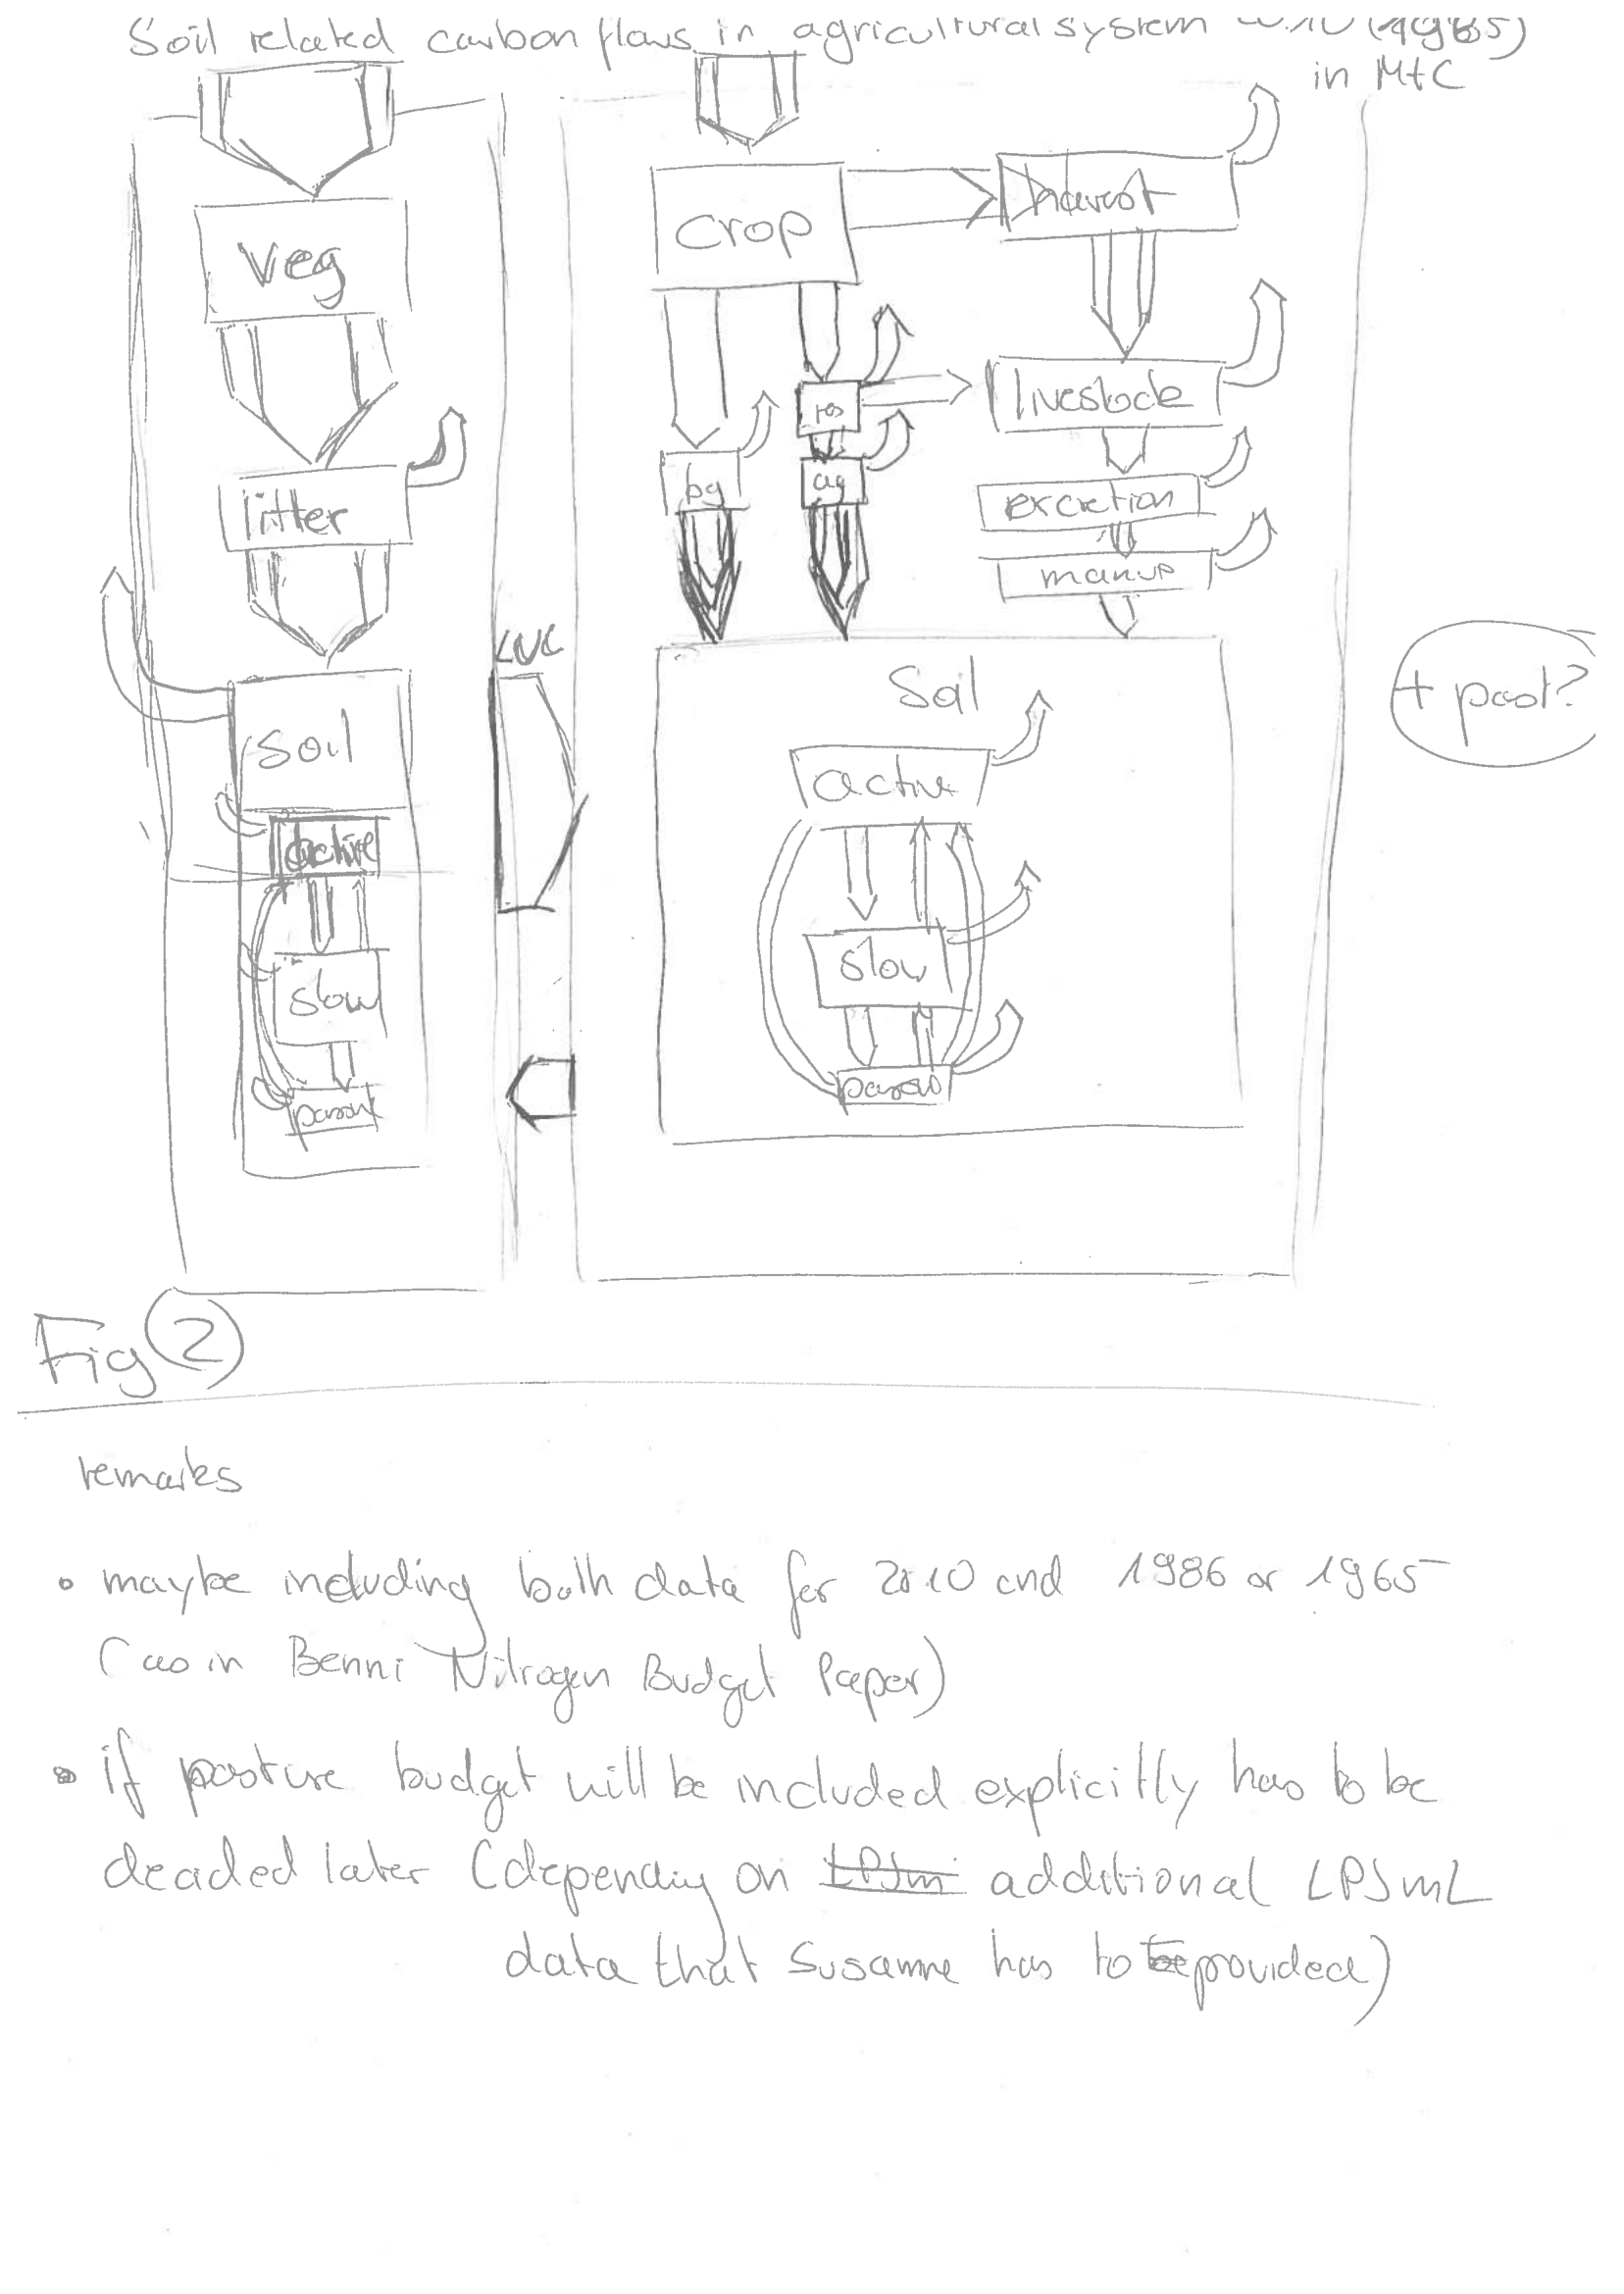
\includegraphics[width=12cm]{images/figs_draft-3} \caption{two column figure}\label{fig:unnamed-chunk-8}
\end{figure}

\begin{figure}
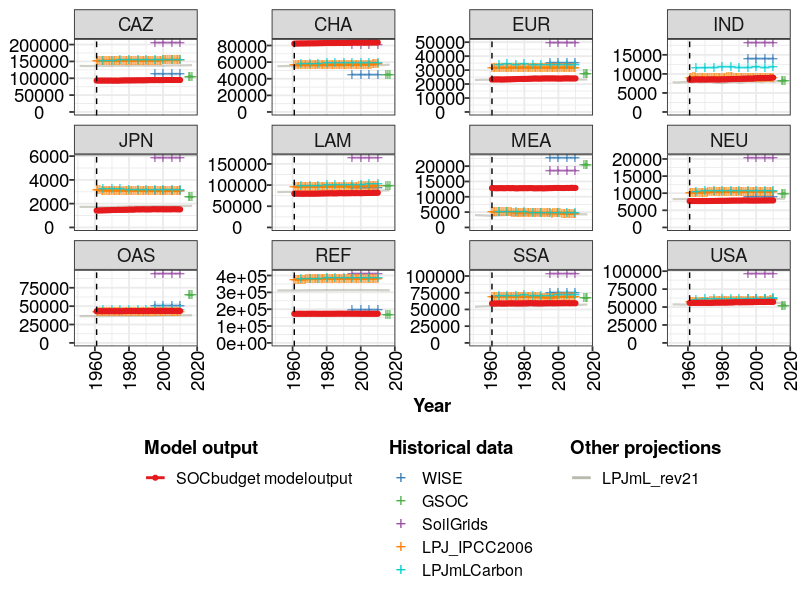
\includegraphics[width=12cm]{images/RegionPlot+Valid} \caption{two column figure}\label{fig:unnamed-chunk-9}
\end{figure}

\begin{figure}
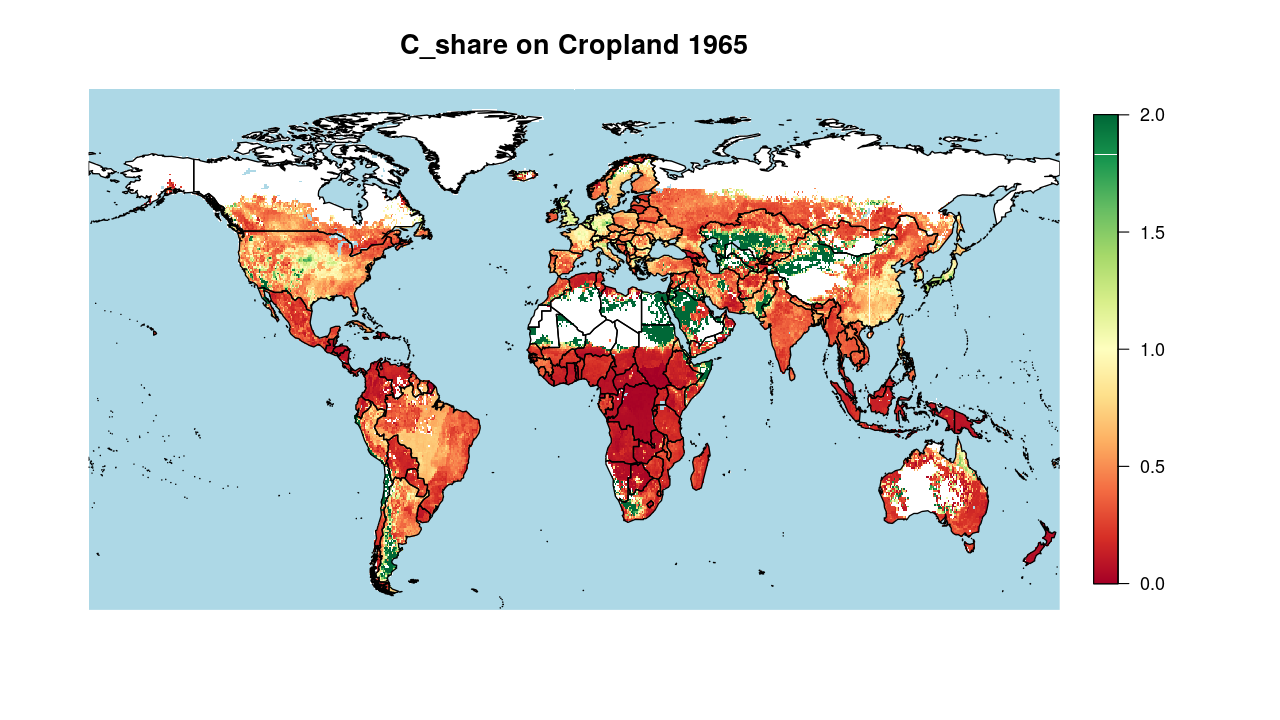
\includegraphics[width=12cm]{images/maps/CShare_1965} 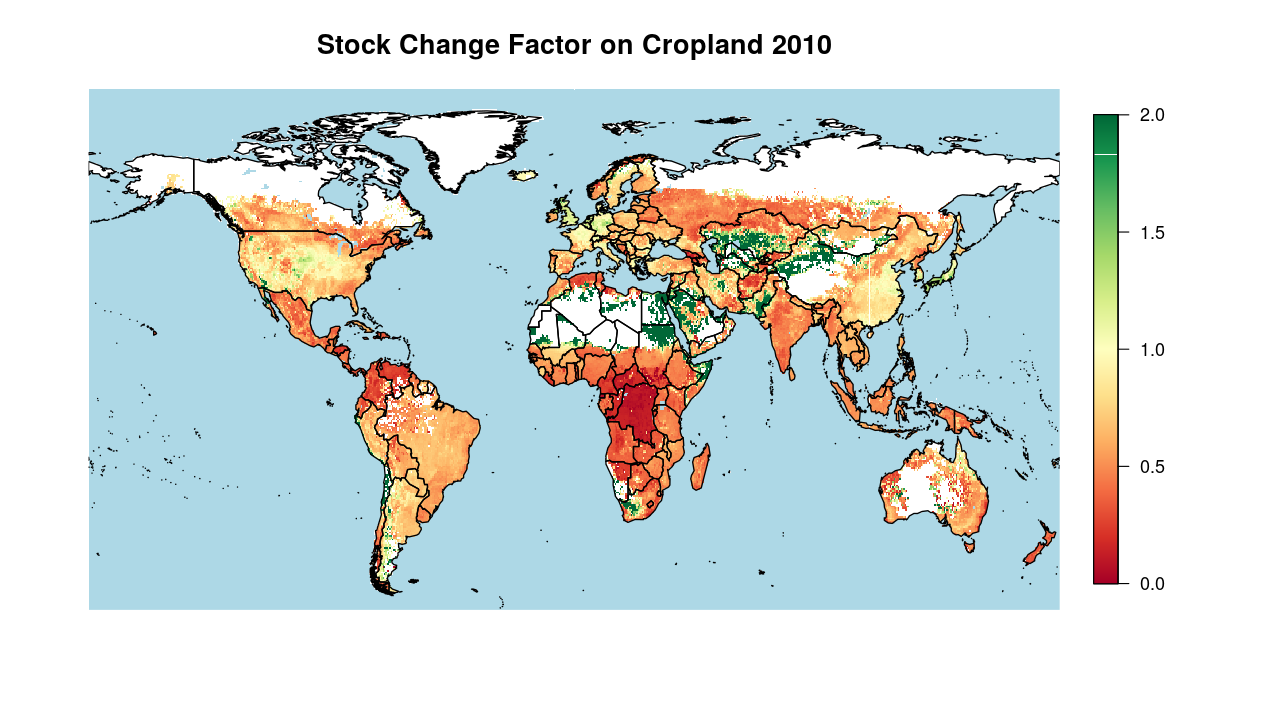
\includegraphics[width=12cm]{images/maps/CShare_2010} \caption{two column figure}\label{fig:unnamed-chunk-10}
\end{figure}

\begin{figure}
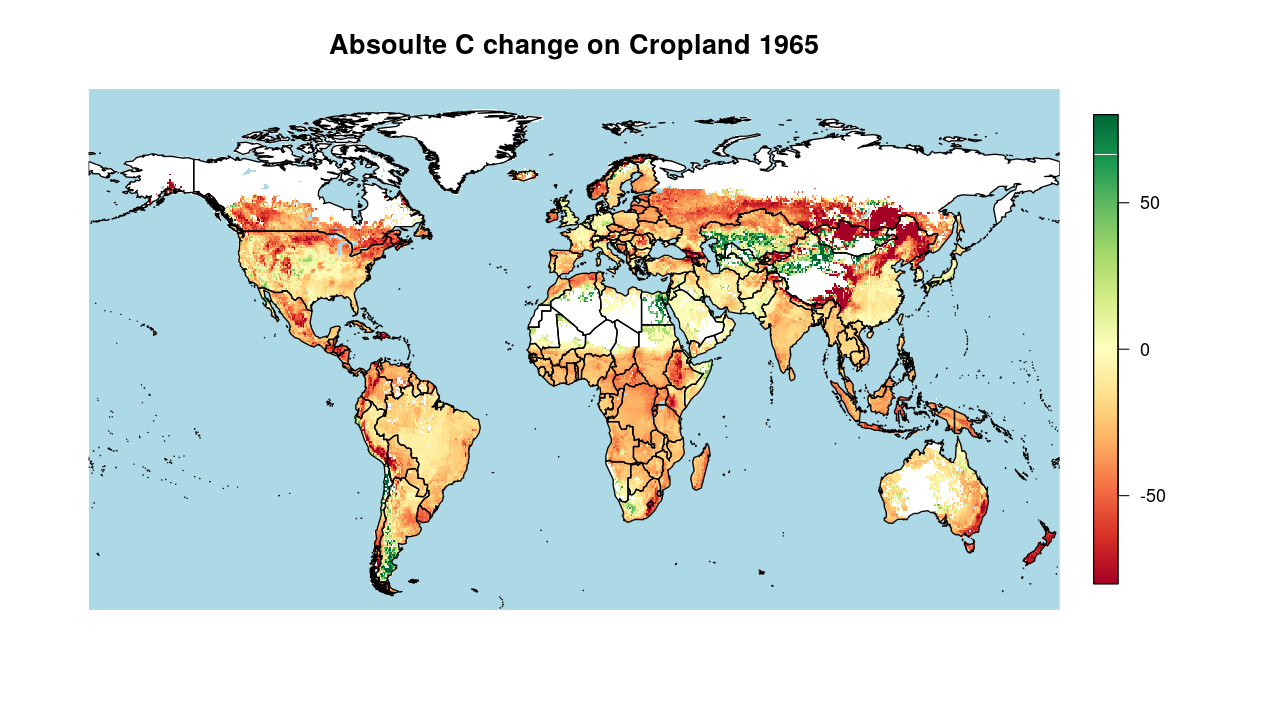
\includegraphics[width=12cm]{images/maps/CIncrease_1965} 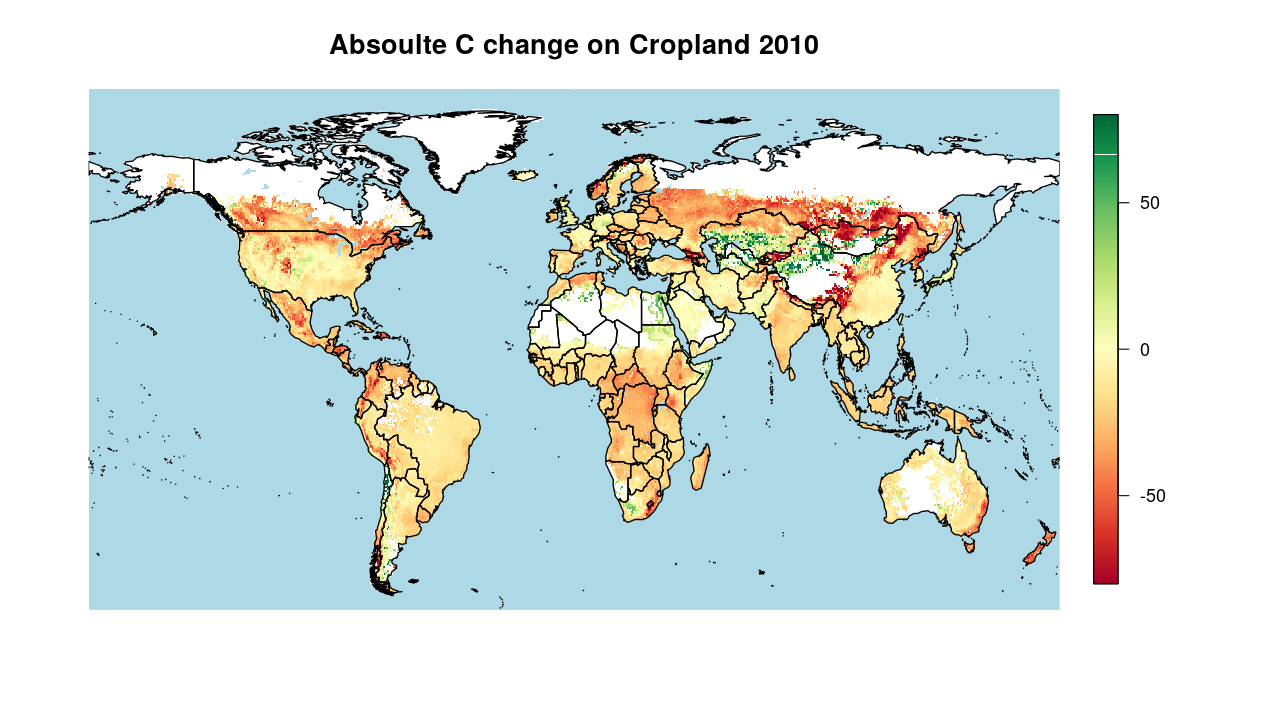
\includegraphics[width=12cm]{images/maps/CIncrease_2010} \caption{two column figure}\label{fig:unnamed-chunk-11}
\end{figure}

\begin{figure}
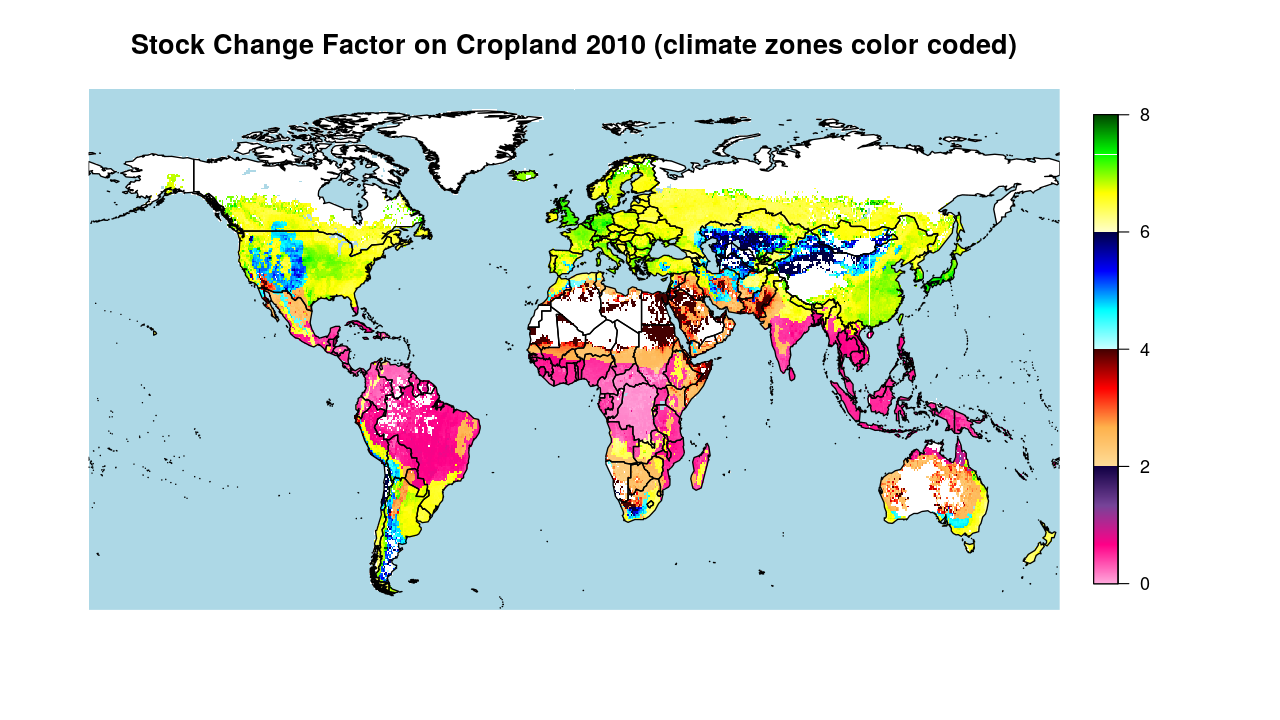
\includegraphics[width=12cm]{images/maps/CShare_4ColorClimates} \caption{one column figure}\label{fig:unnamed-chunk-12}
\end{figure}
\newpage

\section{Discussion}

Shortcommings:

\begin{itemize}
\item
  Carbon displacement via leaching and erosion is neglected in this
  study.
\item
  Non-net/Gross land use transitions are not tracked in this study.
\item
  Within cropland we do not track area transitions, but rather look at
  statistical distributions of the crop functional types. Due to crop
  rotations and missing data on crop specific distributions, these
  transitions would be any way rather uncertain. \newpage
\end{itemize}

\conclusions

The conclusion goes here. You can modify the section name with
\texttt{\textbackslash{}conclusions{[}modified\ heading\ if\ necessary{]}}.
\newpage




\codedataavailability{use this to add a statement when having data sets
and software code
available} %% use this section when having data sets and software code available



%%%%%%%%%%%%%%%%%%%%%%%%%%%%%%%%%%%%%%%%%%
%% optional

%%%%%%%%%%%%%%%%%%%%%%%%%%%%%%%%%%%%%%%%%%
\appendix
\section{Figures and tables in appendices}
\subsection{Option 1}

If you sorted all figures and tables into the sections of the text,
please also sort the appendix figures and appendix tables into the
respective appendix sections. They will be correctly named
automatically.

\subsection{Option 2}

If you put all figures after the reference list, please insert appendix
tables and figures after the normal tables and figures.

\texttt{\textbackslash{}appendixfigures} needs to be added in front of
appendix figures \texttt{\textbackslash{}appendixtables} needs to be
added in front of appendix tables

Please add \texttt{\textbackslash{}clearpage} between each table and/or
figure. Further guidelines on figures and tables can be found below.
Regarding figures and tables in appendices, the following two options
are possible depending on your general handling of figures and tables in
the manuscript environment: To rename them correctly to A1, A2, etc.,
please add the following commands in front of them:
\noappendix

%%%%%%%%%%%%%%%%%%%%%%%%%%%%%%%%%%%%%%%%%%
\authorcontribution{Karstens wrote code and paper build on work of
Bodirsky. Bodirsky and Popp revised paper.} %% optional section

%%%%%%%%%%%%%%%%%%%%%%%%%%%%%%%%%%%%%%%%%%
\competinginterests{The authors declare no competing
interests.} %% this section is mandatory even if you declare that no competing interests are present

%%%%%%%%%%%%%%%%%%%%%%%%%%%%%%%%%%%%%%%%%%
\disclaimer{We like Copernicus.} %% optional section

%%%%%%%%%%%%%%%%%%%%%%%%%%%%%%%%%%%%%%%%%%
\begin{acknowledgements}
Thanks to the rticles contributors!
\end{acknowledgements}

%% REFERENCES
%% DN: pre-configured to BibTeX for rticles

%% The reference list is compiled as follows:
%%
%% \begin{thebibliography}{}
%%
%% \bibitem[AUTHOR(YEAR)]{LABEL1}
%% REFERENCE 1
%%
%% \bibitem[AUTHOR(YEAR)]{LABEL2}
%% REFERENCE 2
%%
%% \end{thebibliography}

%% Since the Copernicus LaTeX package includes the BibTeX style file copernicus.bst,
%% authors experienced with BibTeX only have to include the following two lines:
%%
\bibliographystyle{copernicus}
\bibliography{SOCbudget.bib}
%%
%% URLs and DOIs can be entered in your BibTeX file as:
%%
%% URL = {http://www.xyz.org/~jones/idx_g.htm}
%% DOI = {10.5194/xyz}


%% LITERATURE CITATIONS
%%
%% command                        & example result
%% \citet{jones90}|               & Jones et al. (1990)
%% \citep{jones90}|               & (Jones et al., 1990)
%% \citep{jones90,jones93}|       & (Jones et al., 1990, 1993)
%% \citep[p.~32]{jones90}|        & (Jones et al., 1990, p.~32)
%% \citep[e.g.,][]{jones90}|      & (e.g., Jones et al., 1990)
%% \citep[e.g.,][p.~32]{jones90}| & (e.g., Jones et al., 1990, p.~32)
%% \citeauthor{jones90}|          & Jones et al.
%% \citeyear{jones90}|            & 1990

\end{document}
